\documentclass[10pt]{article}

\usepackage[a4paper,left=20mm, right=20mm, top=20mm, bottom=20mm]{geometry}
\usepackage{pdfpages}
\usepackage{markdown}
\usepackage{multicol}
\usepackage{caption}

\title{2-way Concrete Speaker Documentation}
\author{Eero Talus}
\date{\today}

\begin{document}
\maketitle
\tableofcontents

\section{Introduction}

\noindent This PDF contains documentation for my self designed vented two way
speakers. All the design files can be found from the GIT repository at
\url{https://github.com/eerotal/2-way-speaker}.\\

\noindent The speaker specifications are:

\begin{itemize}
\item Cabinet volume (V): 20 l
\item Cabinet tuning frequenxy (Fb): 42.49 Hz
\item Woofer: Visaton W-170 S 8Ohm
\item Tweeter: Visaton SC-10 N
\end{itemize}

\noindent The speaker cabinet was designed to have a frequency response that's
as flat as possible over the entire bandwidth of the speaker. The cabinet
features a theoretically optimal reflex port designed based on various research
papers on the subject. The cabinet is constructed from concrete and wood to
increase its mass and to improve speaker performance.\\

\noindent The speaker uses a crossover circuit made using third order
Butterworth filters. Speaker impedance and sensitivity matching was also taken
into account while desiging the filter. All design and documentation files were
created using open file formats, tools and technologies.\\

\noindent You can run the shell script \texttt makedocs.sh to generate this
PDF file.

\section{Respository directory structure}

\begin{itemize}
\item 2-way-speaker
    \begin{itemize}
    \item crossover
        \begin{itemize}
        \item KiCad
            \begin{itemize}
            \item \textit{Crossover schematics and PCB design files.}
            \end{itemize}
        \item ngspice
            \begin{itemize}
            \item \textit{NgSpice crossover simulation files.}
            \end{itemize}
        \end{itemize}
    \item docs
        \begin{itemize}
        \item \textit{Documentation files.}
        \end{itemize}
    \item latex
        \begin{itemize}
        \item \textit{LaTeX files for concatenating all documentation files into one PDF.}
        \end{itemize}
    \item math
        \begin{itemize}
        \item \textit{WxMaxima design calculations.}
        \end{itemize}
    \item models
        \begin{itemize}
        \item \textit{FreeCAD 3D design files.}
        \end{itemize}
    \item simulation
        \begin{itemize}
        \item \textit{Visaton Boxsim simulation files.}
        \end{itemize}
    \end{itemize}
\end{itemize}

\section{Software and technologies}

Below is a list of the software and technologies used in this project.

\begin{itemize}
\item KiCad: Crossover electronics design.
\item ngspice: Crossover circuit simulation.
\item FreeCAD: 3D models and mechanical drawings.
\item Boxsim: Speaker simulation.
\item wxMaxima: Design calculations.
\item LaTeX: Documentation
\end{itemize}

\section{License}

\noindent The contents of this repository are licensed under the INSERT
LICENSE license unless otherwise noted. The full license text is included in
the file \texttt LICENSE.txt in the root of the repository.

\pagebreak
\null
\vfil
\centering\section{Mechanical drawings}
\vfil
\pagebreak
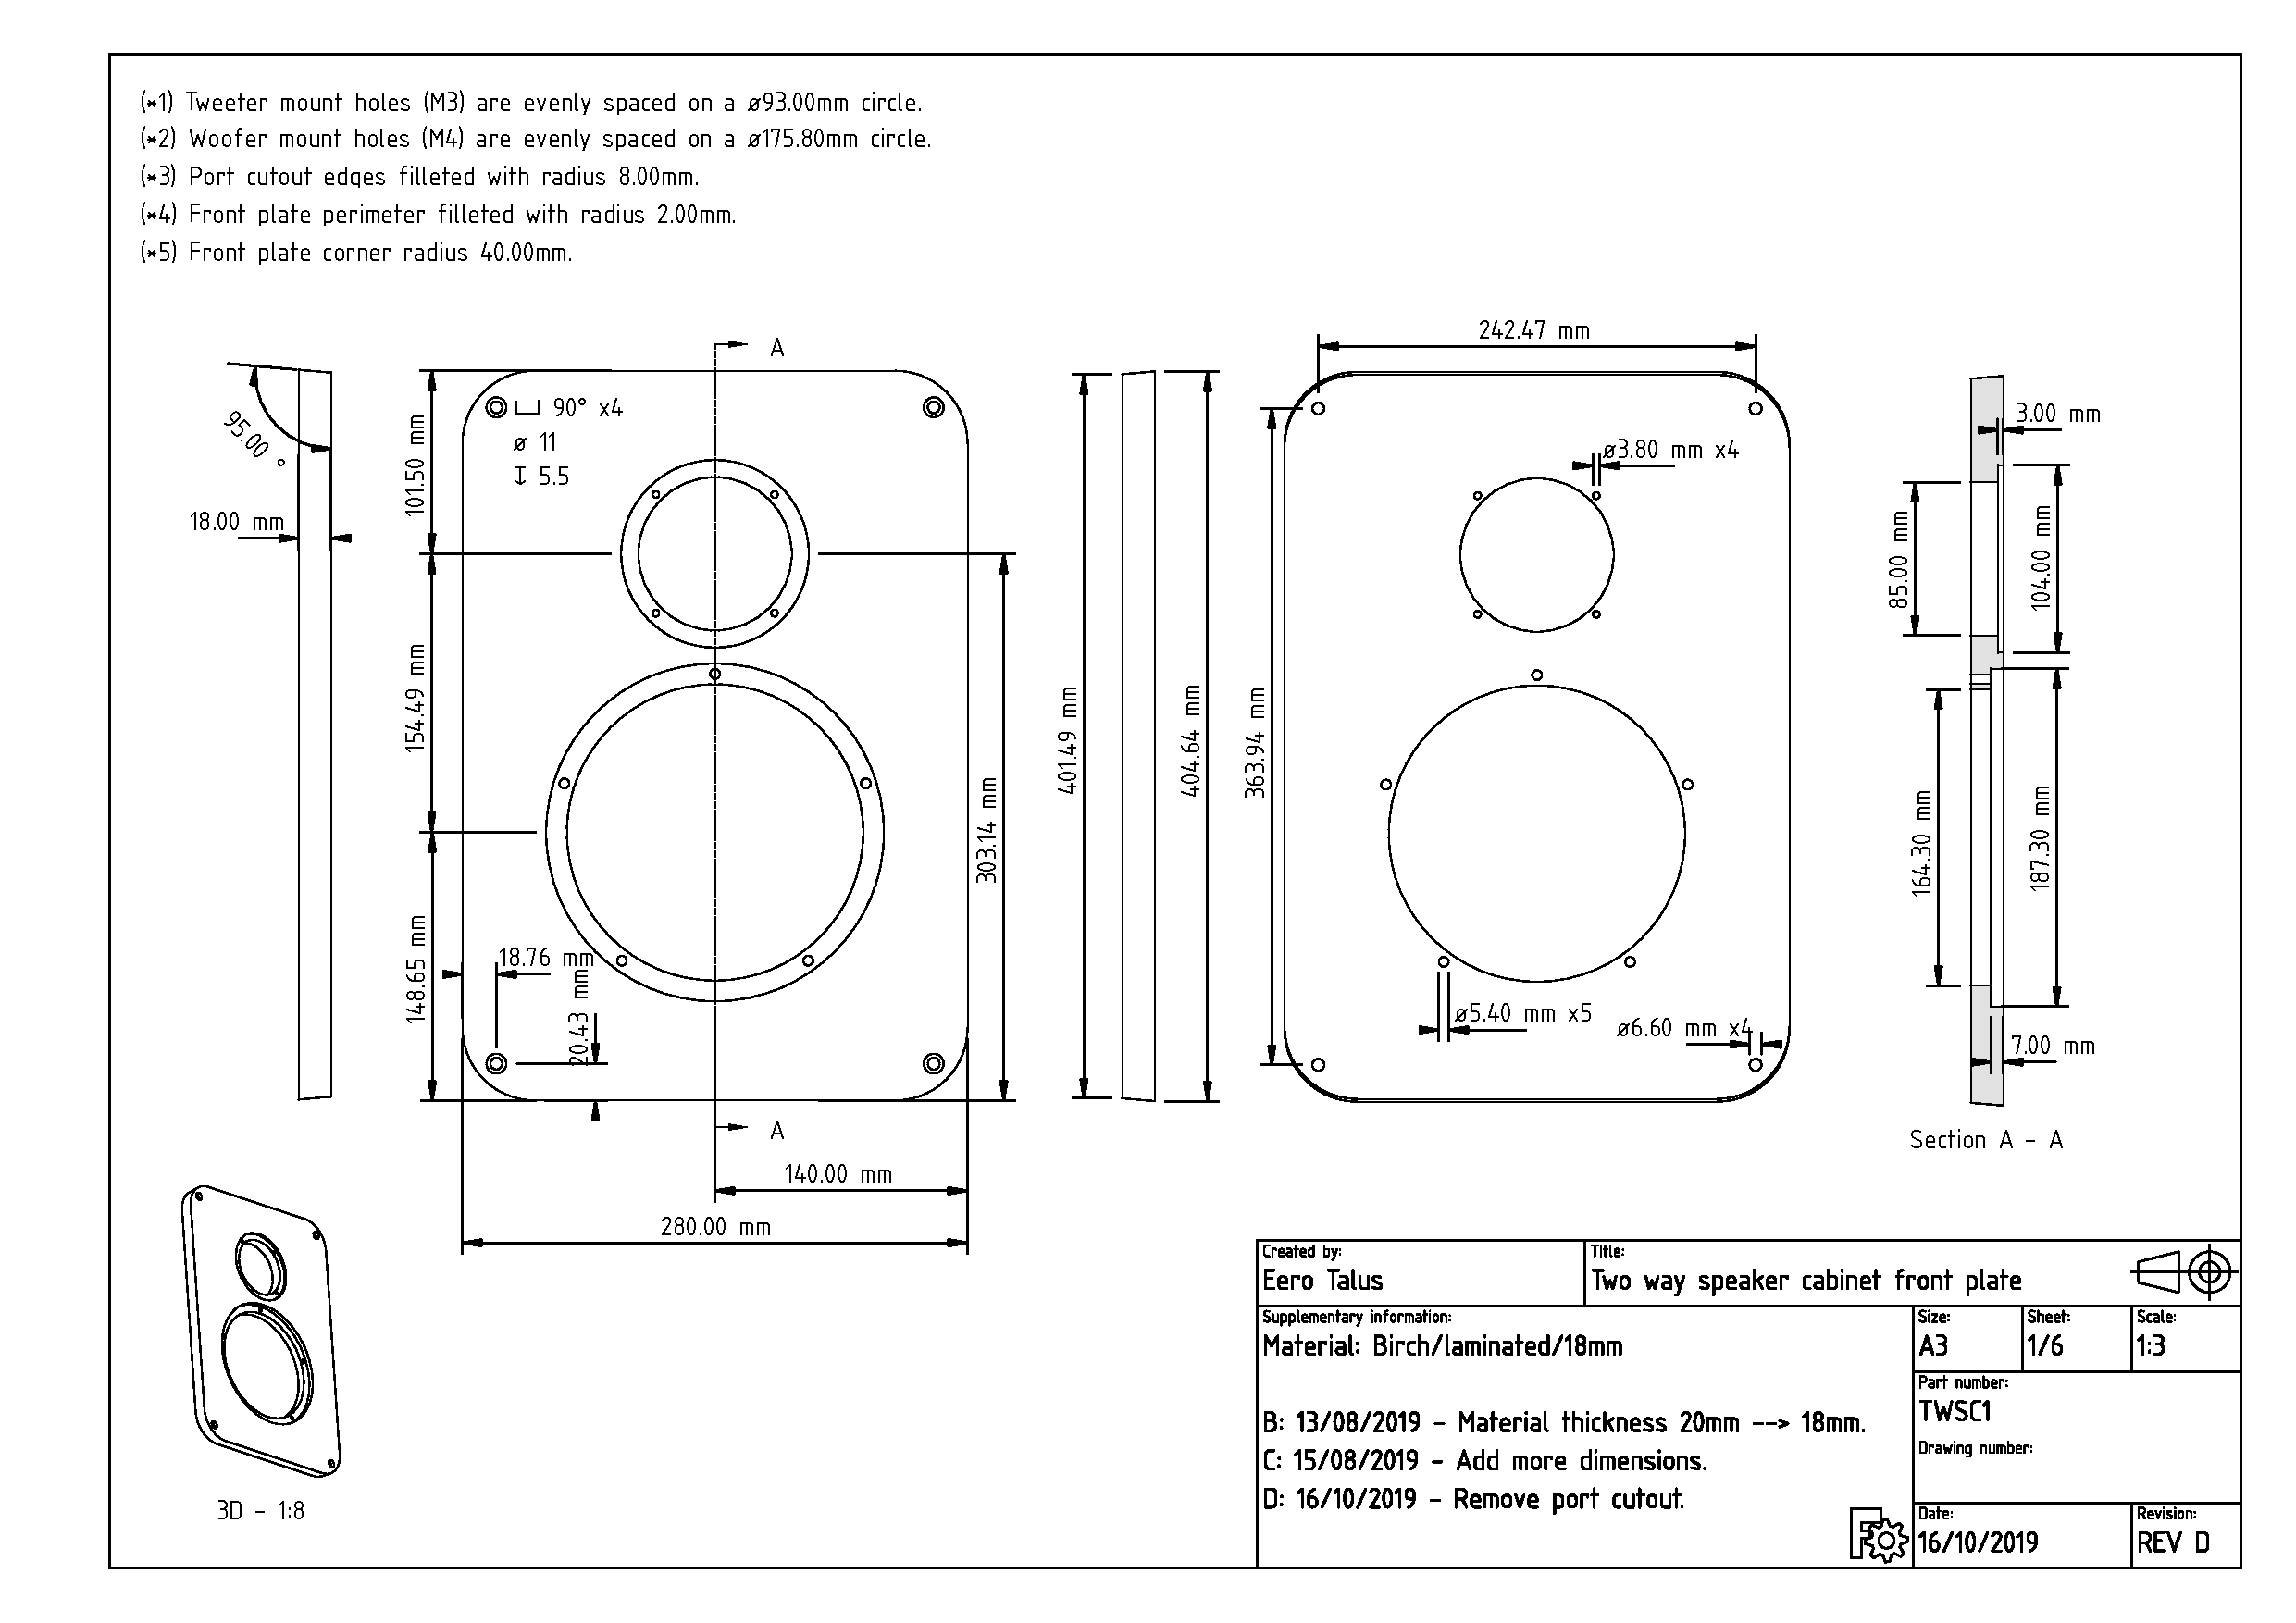
\includepdf[landscape=true]{../drawings/Front_Plate_Drawing.pdf}
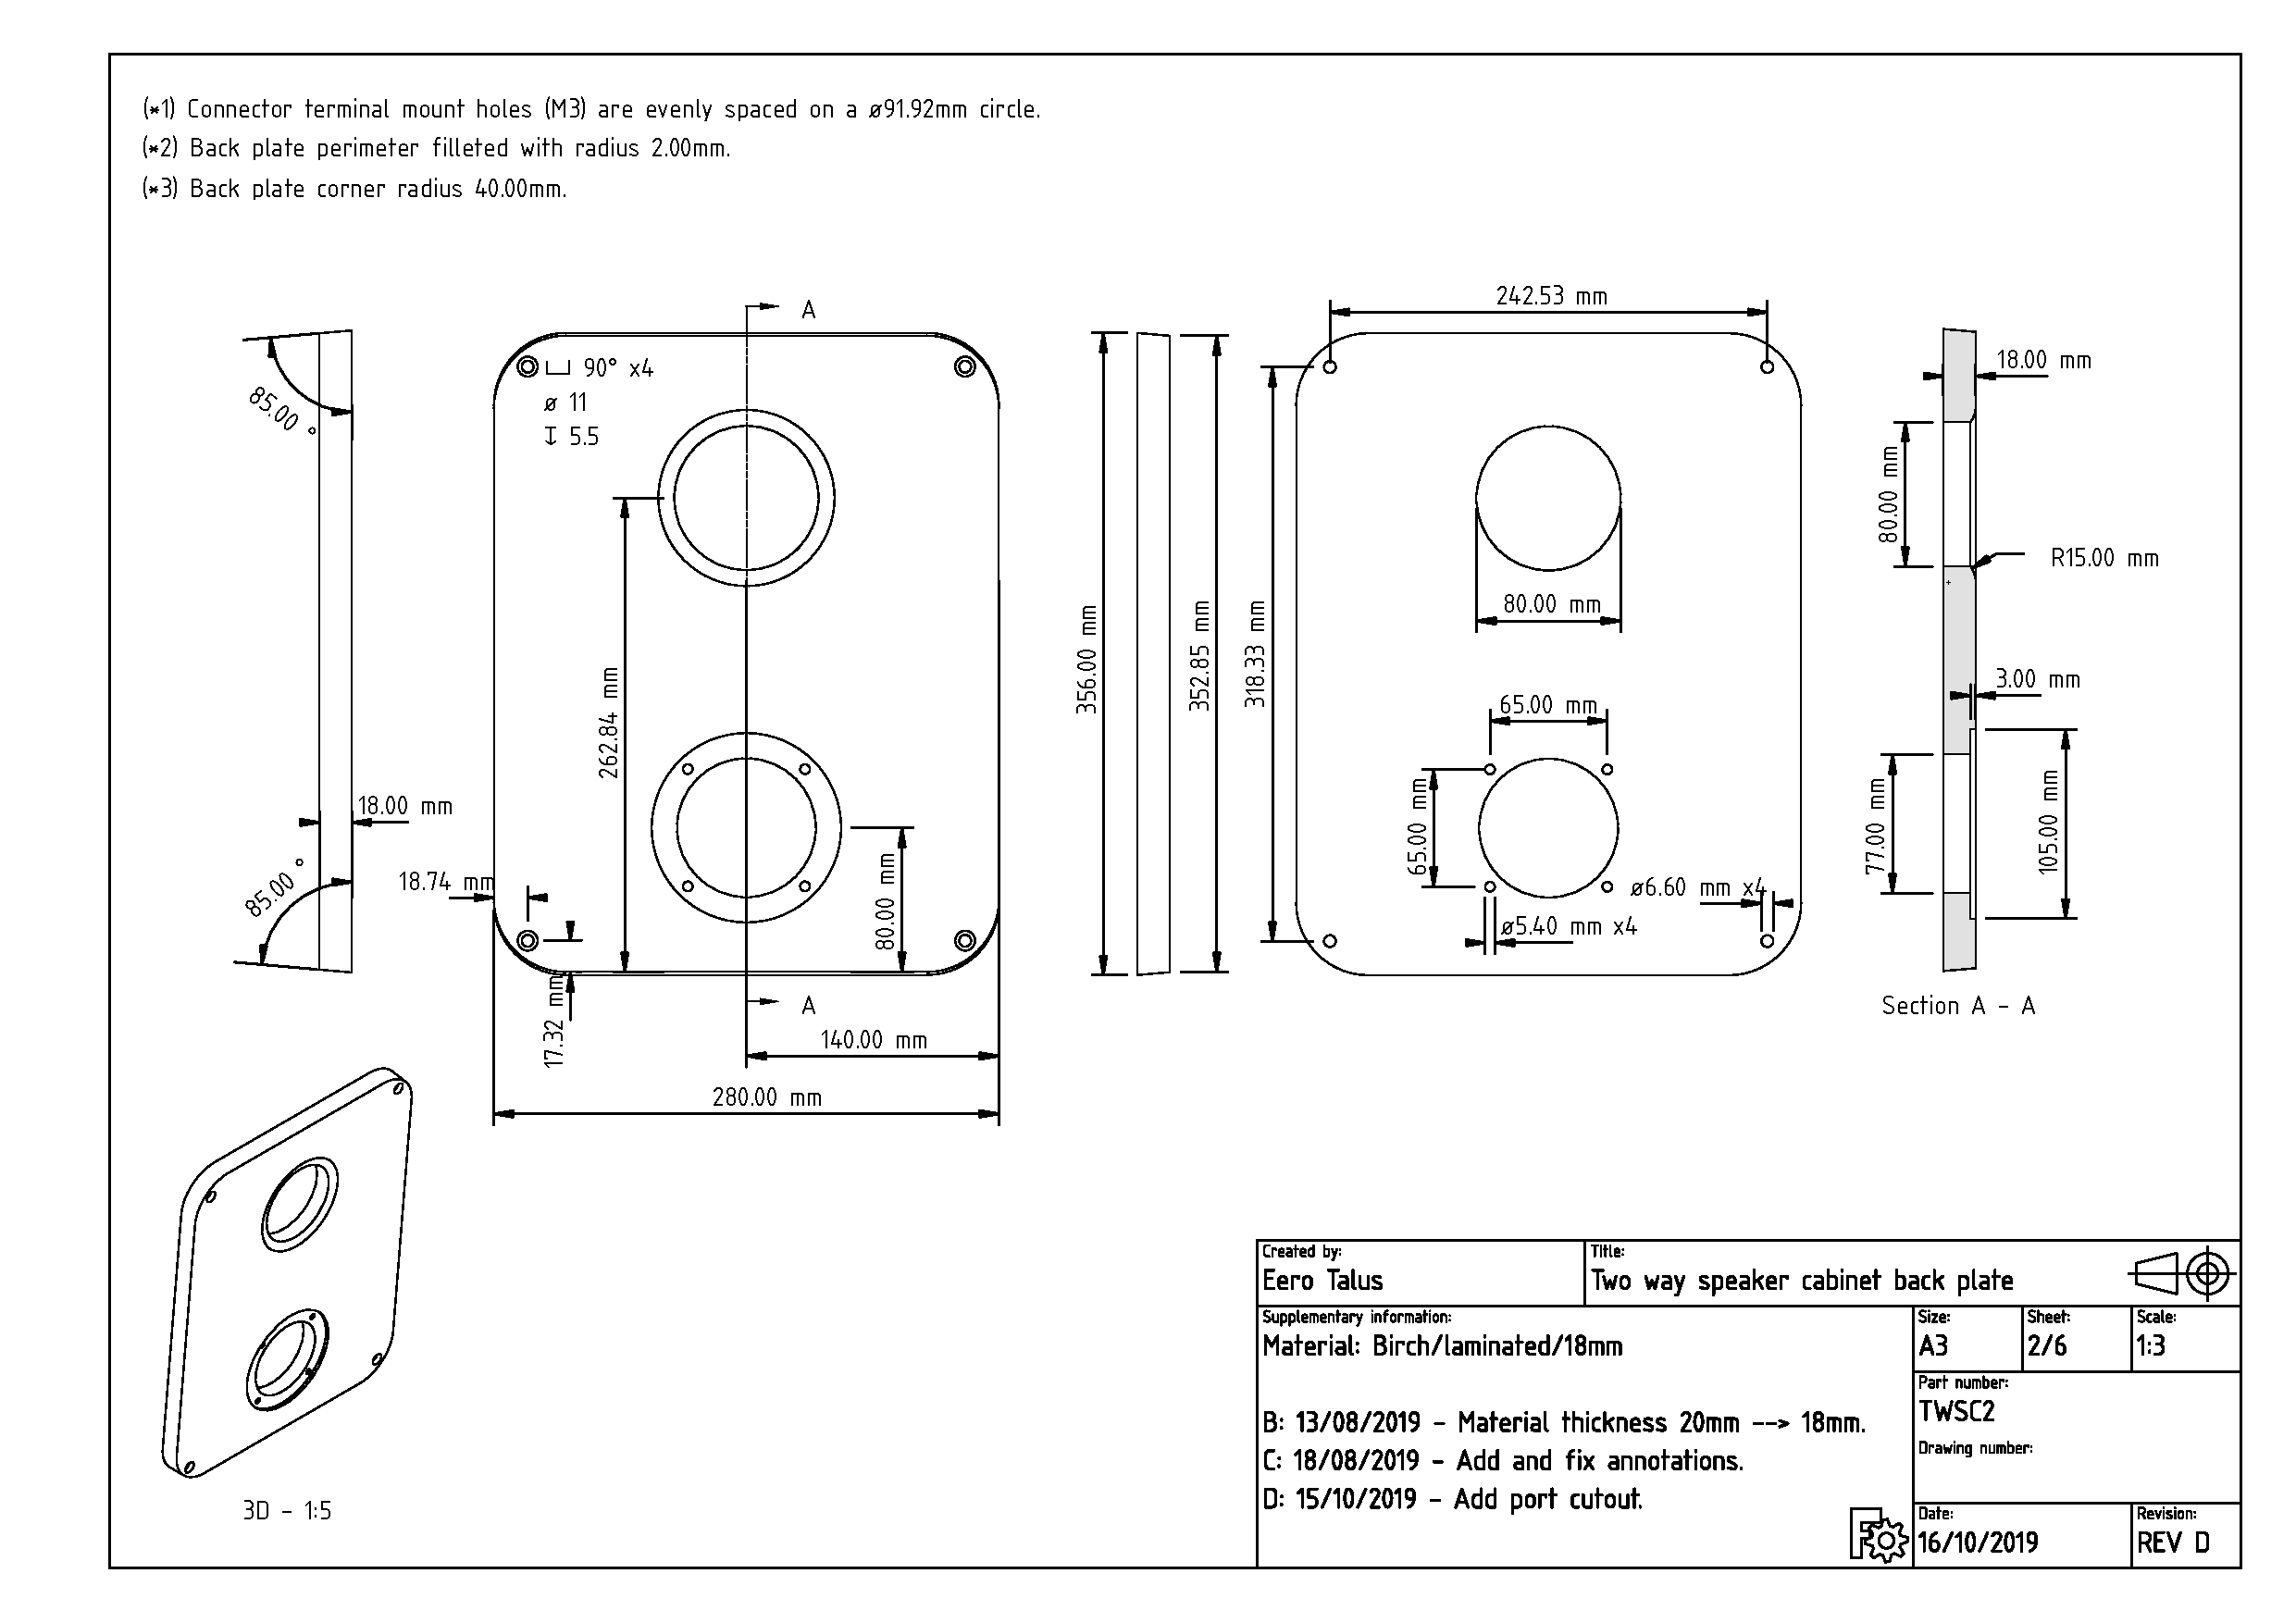
\includepdf[landscape=true]{../drawings/Back_Plate_Drawing.pdf}
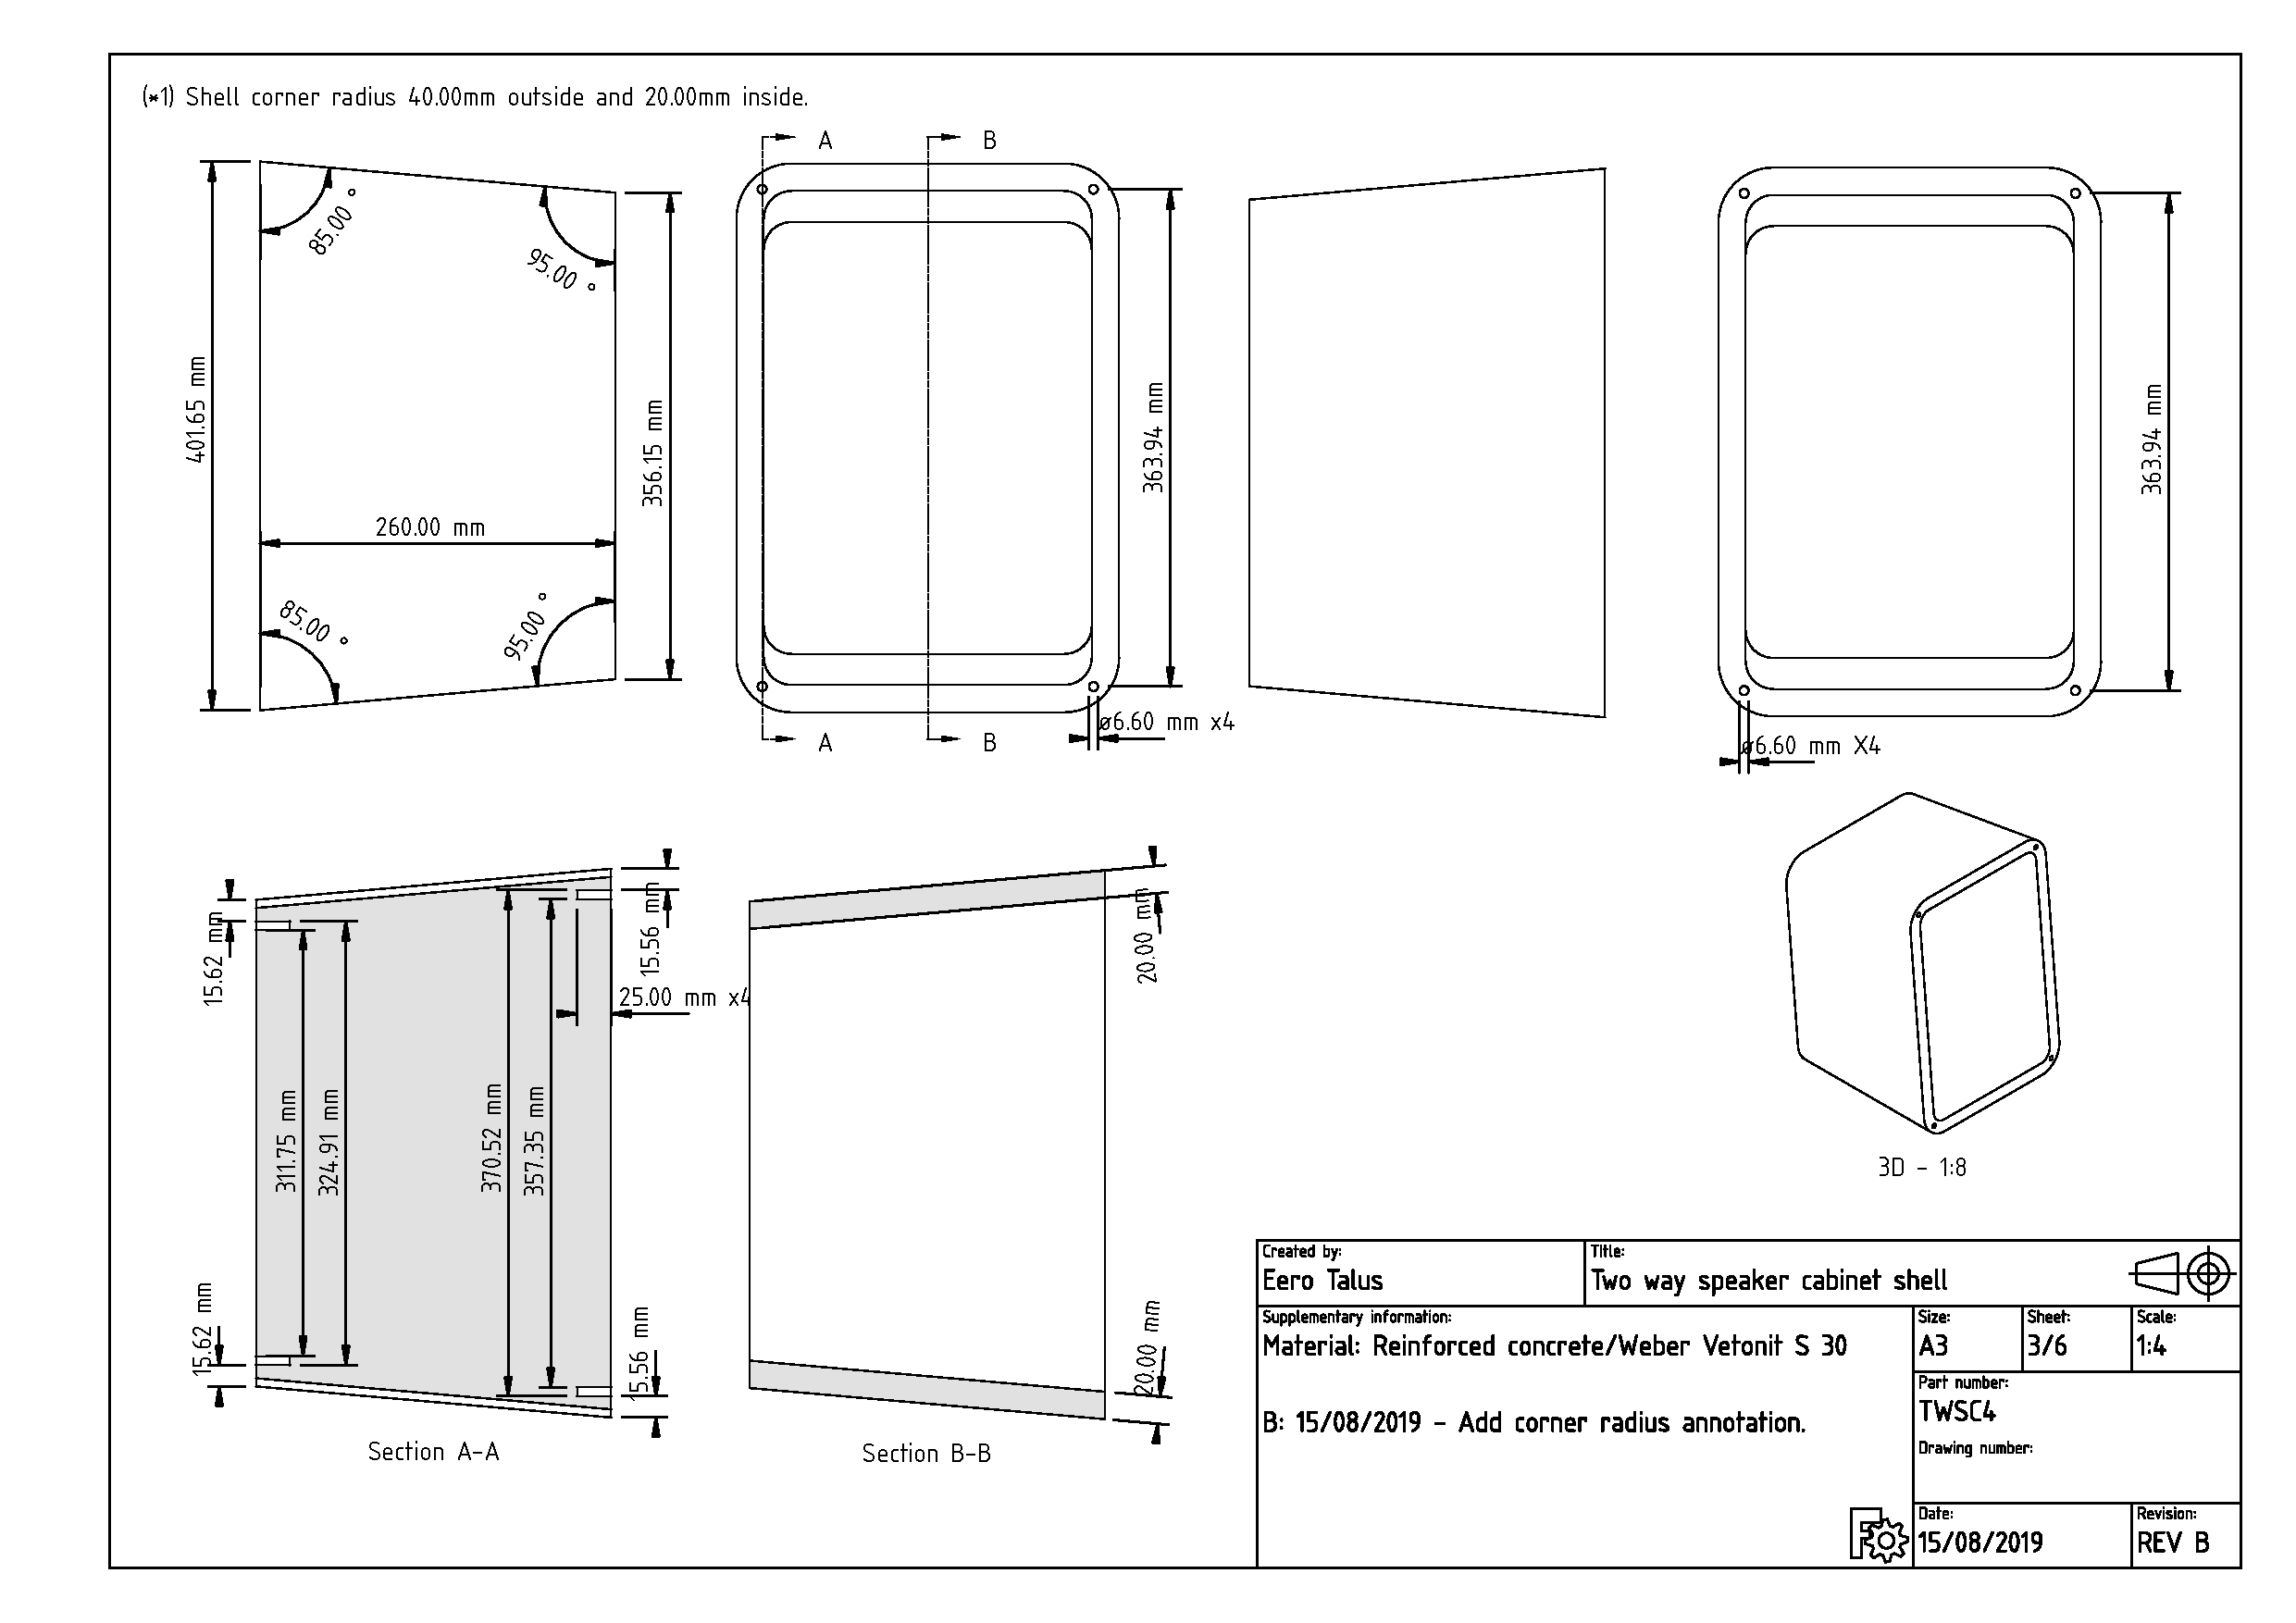
\includepdf[landscape=true]{../drawings/Shell_Drawing.pdf}
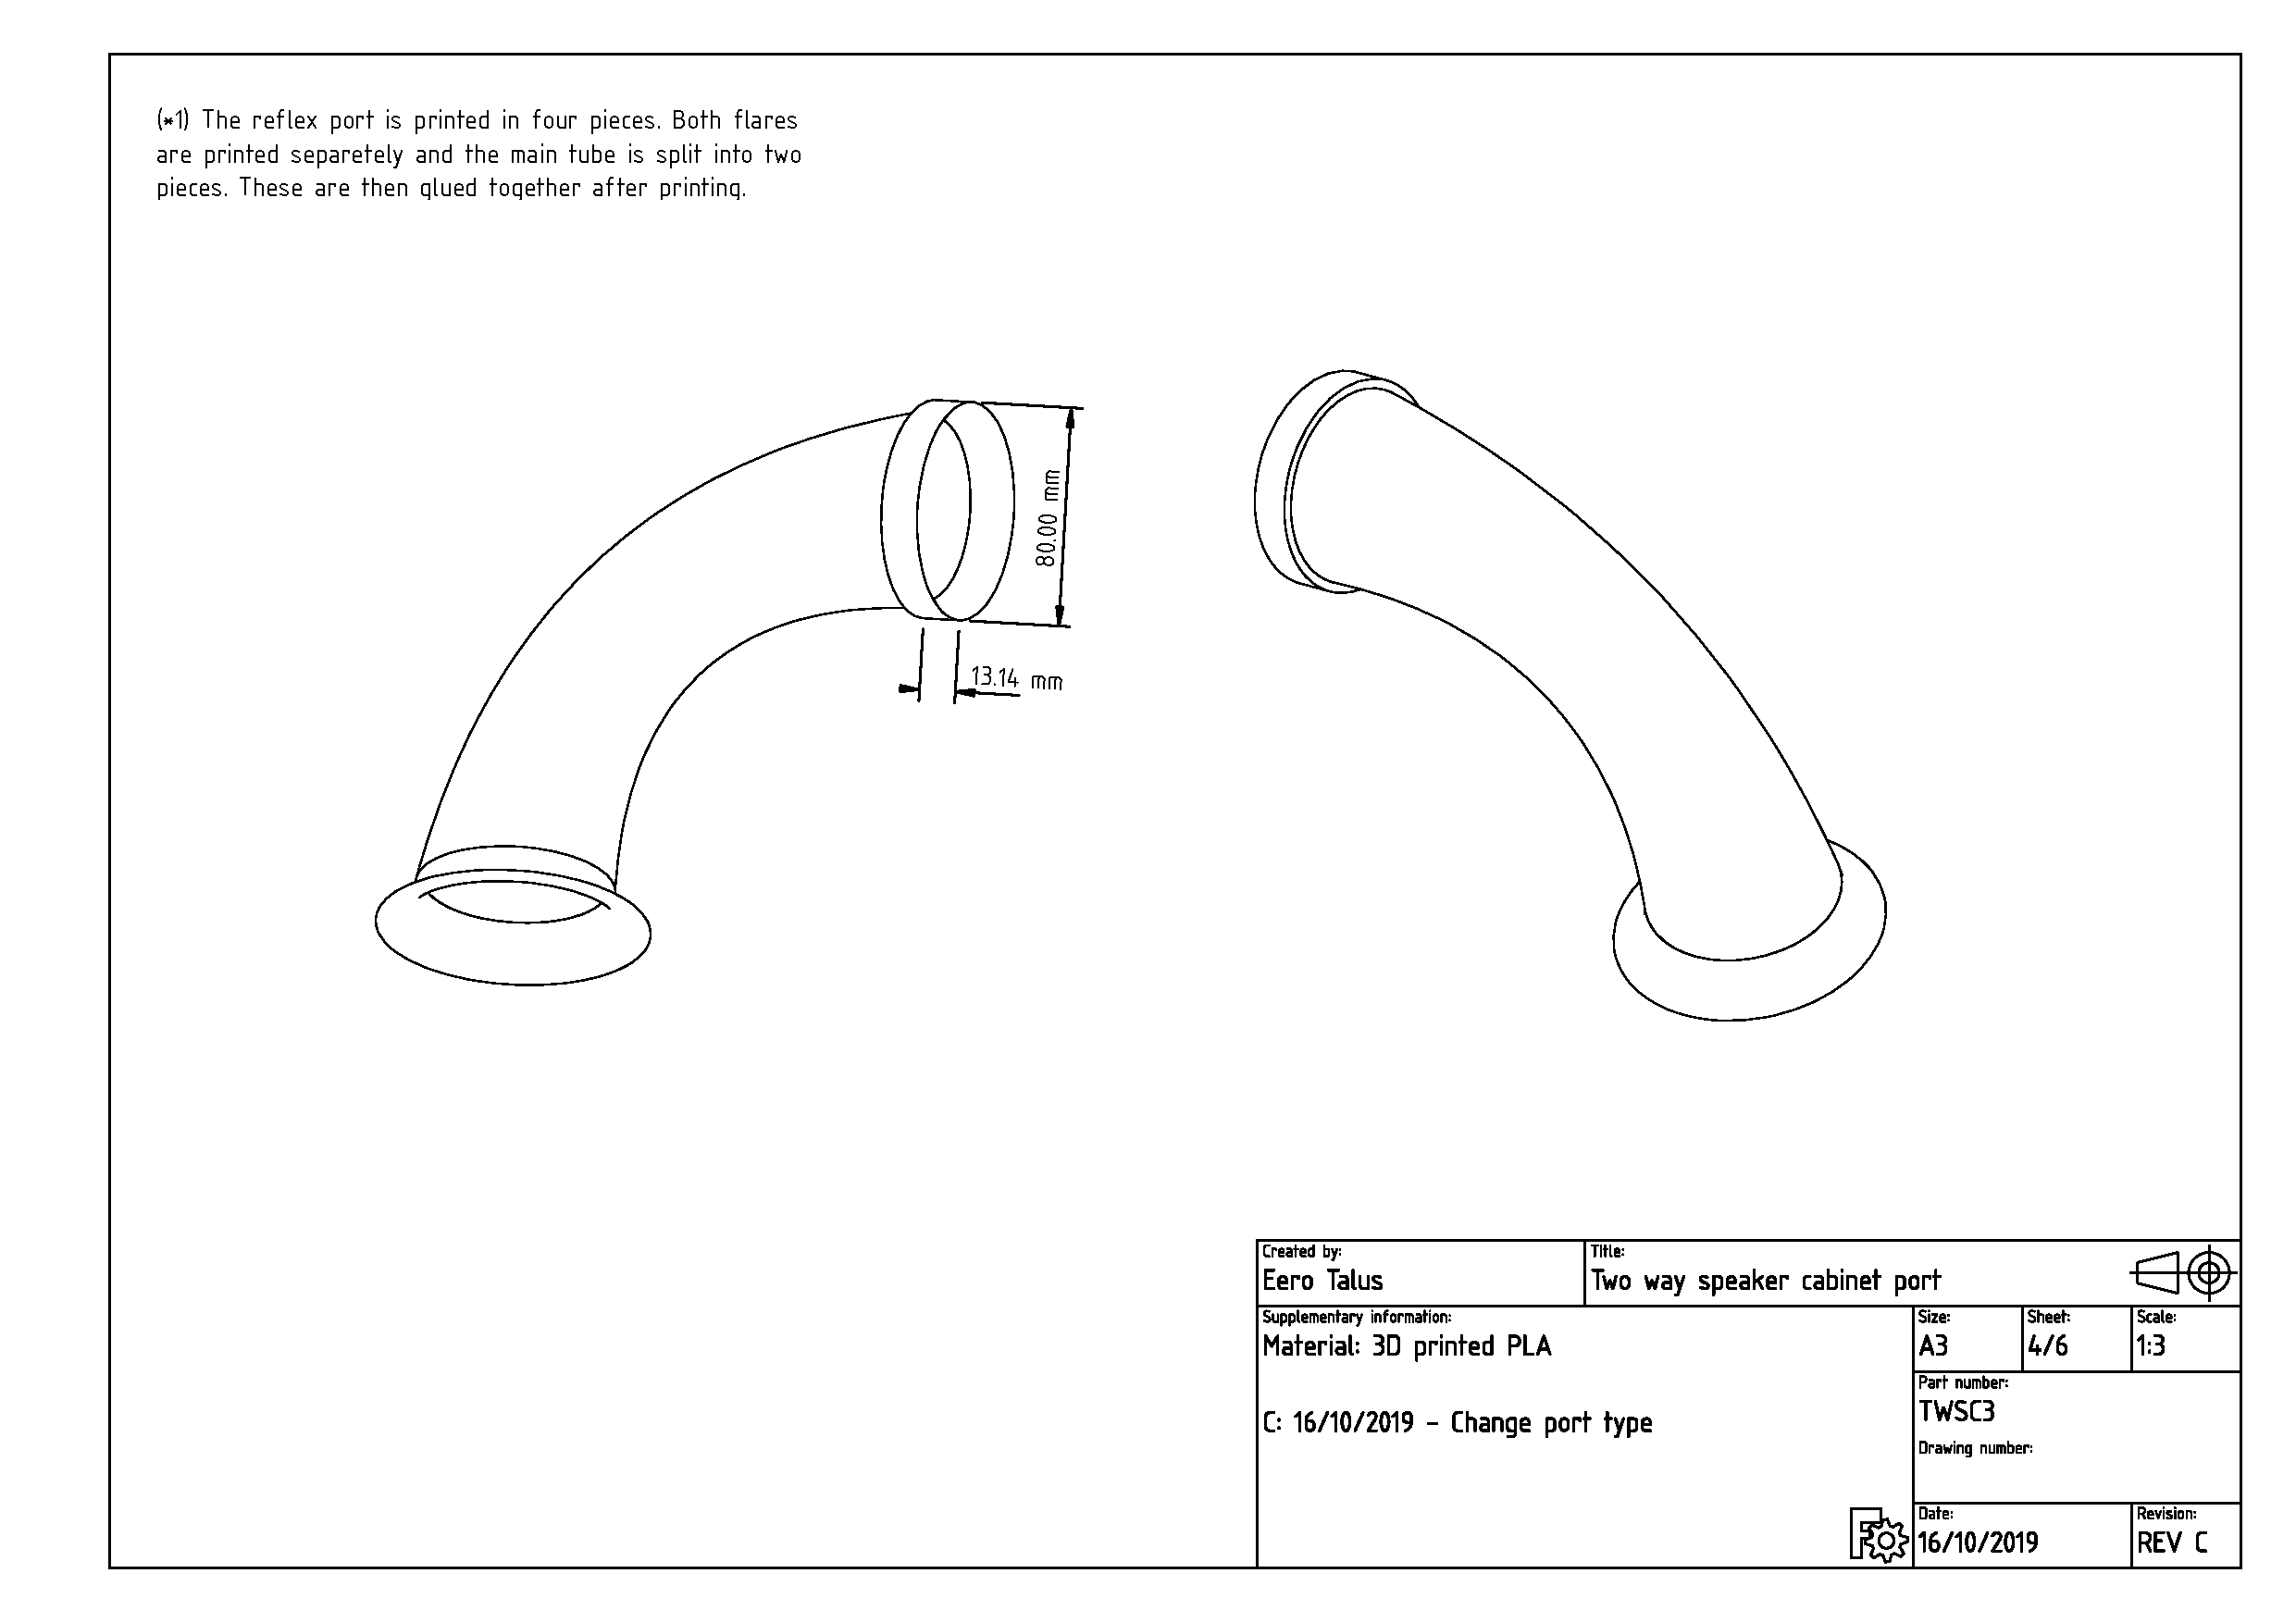
\includepdf[landscape=true]{../drawings/Port_Drawing.pdf}

\pagebreak
\null
\vfil
\centering\section{Crossover simulation graphs}
\vfil
\pagebreak
\begin{multicols}{2}
	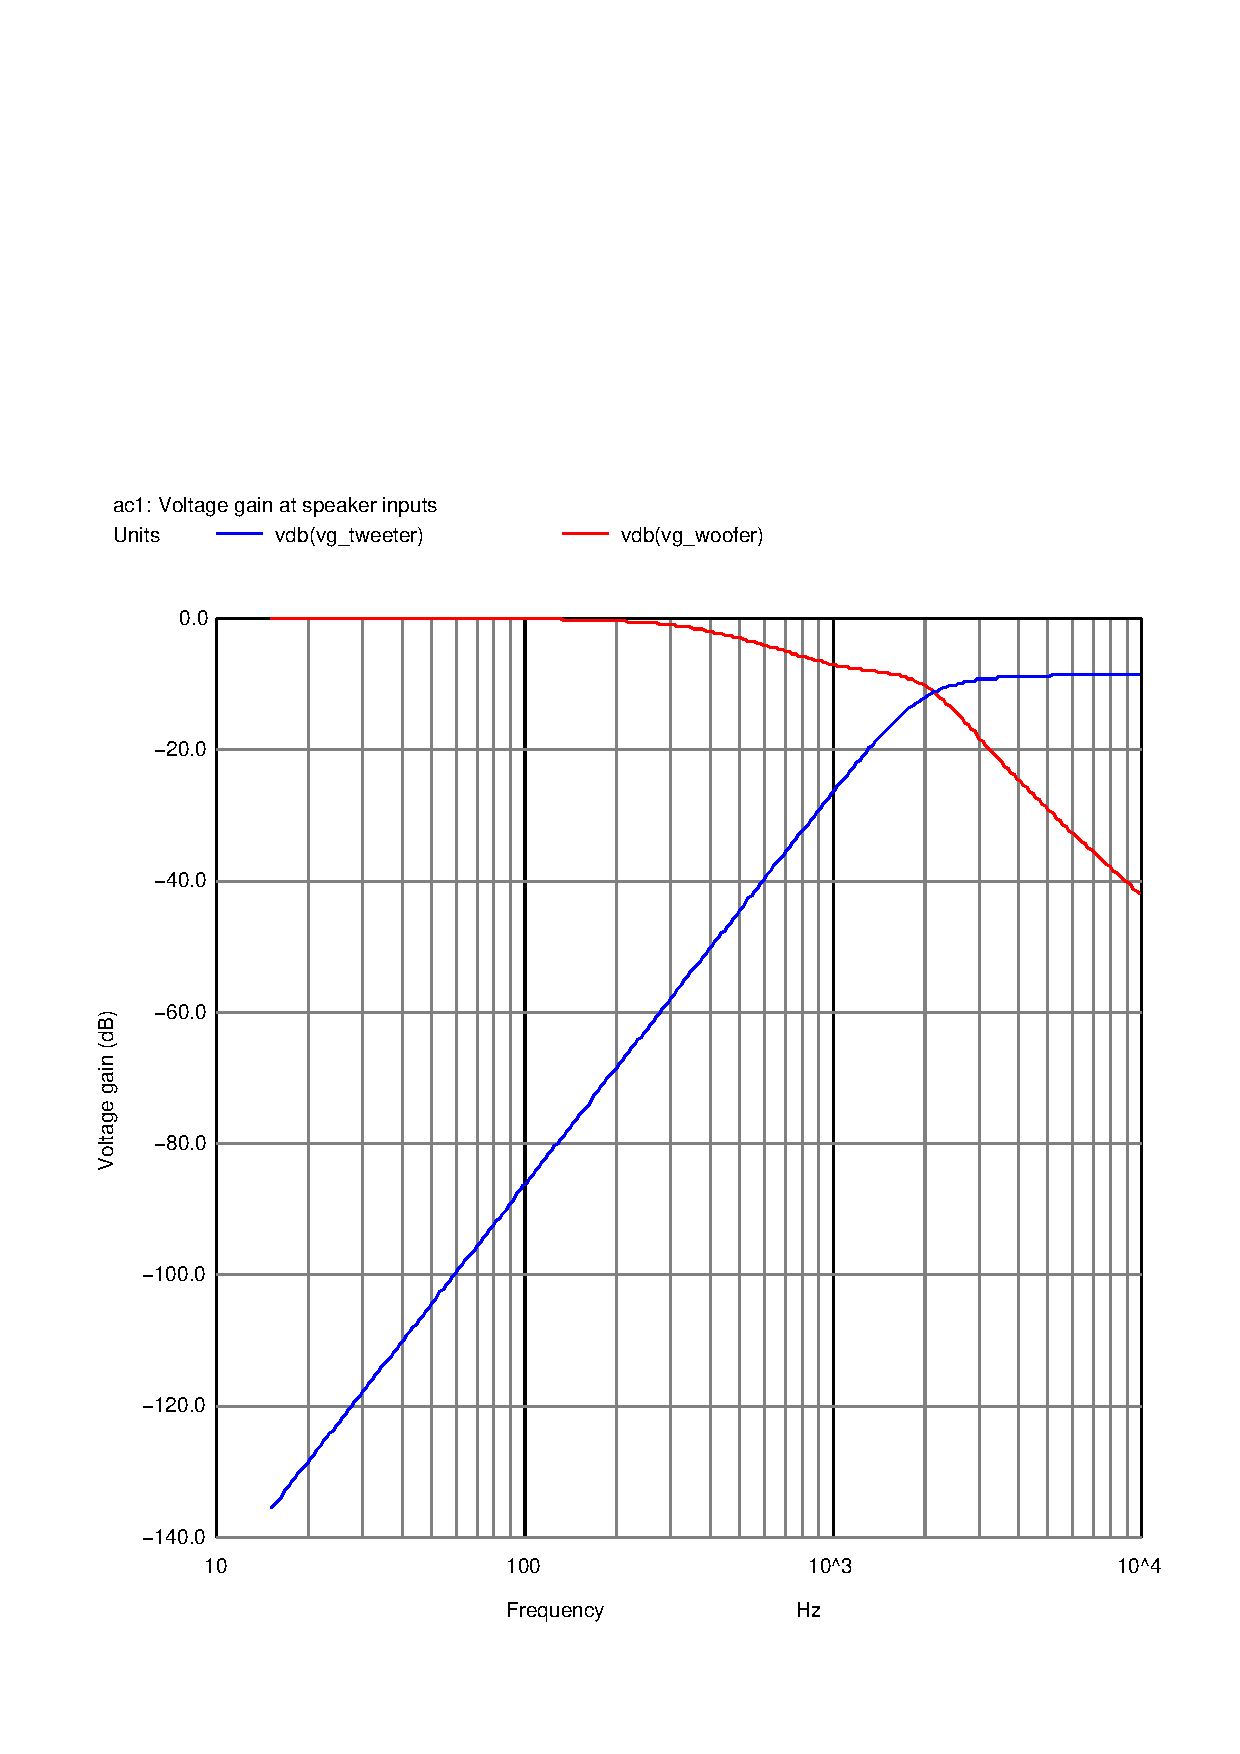
\includegraphics[scale=0.35,page=1]{../crossover/ngspice/gain.pdf}
	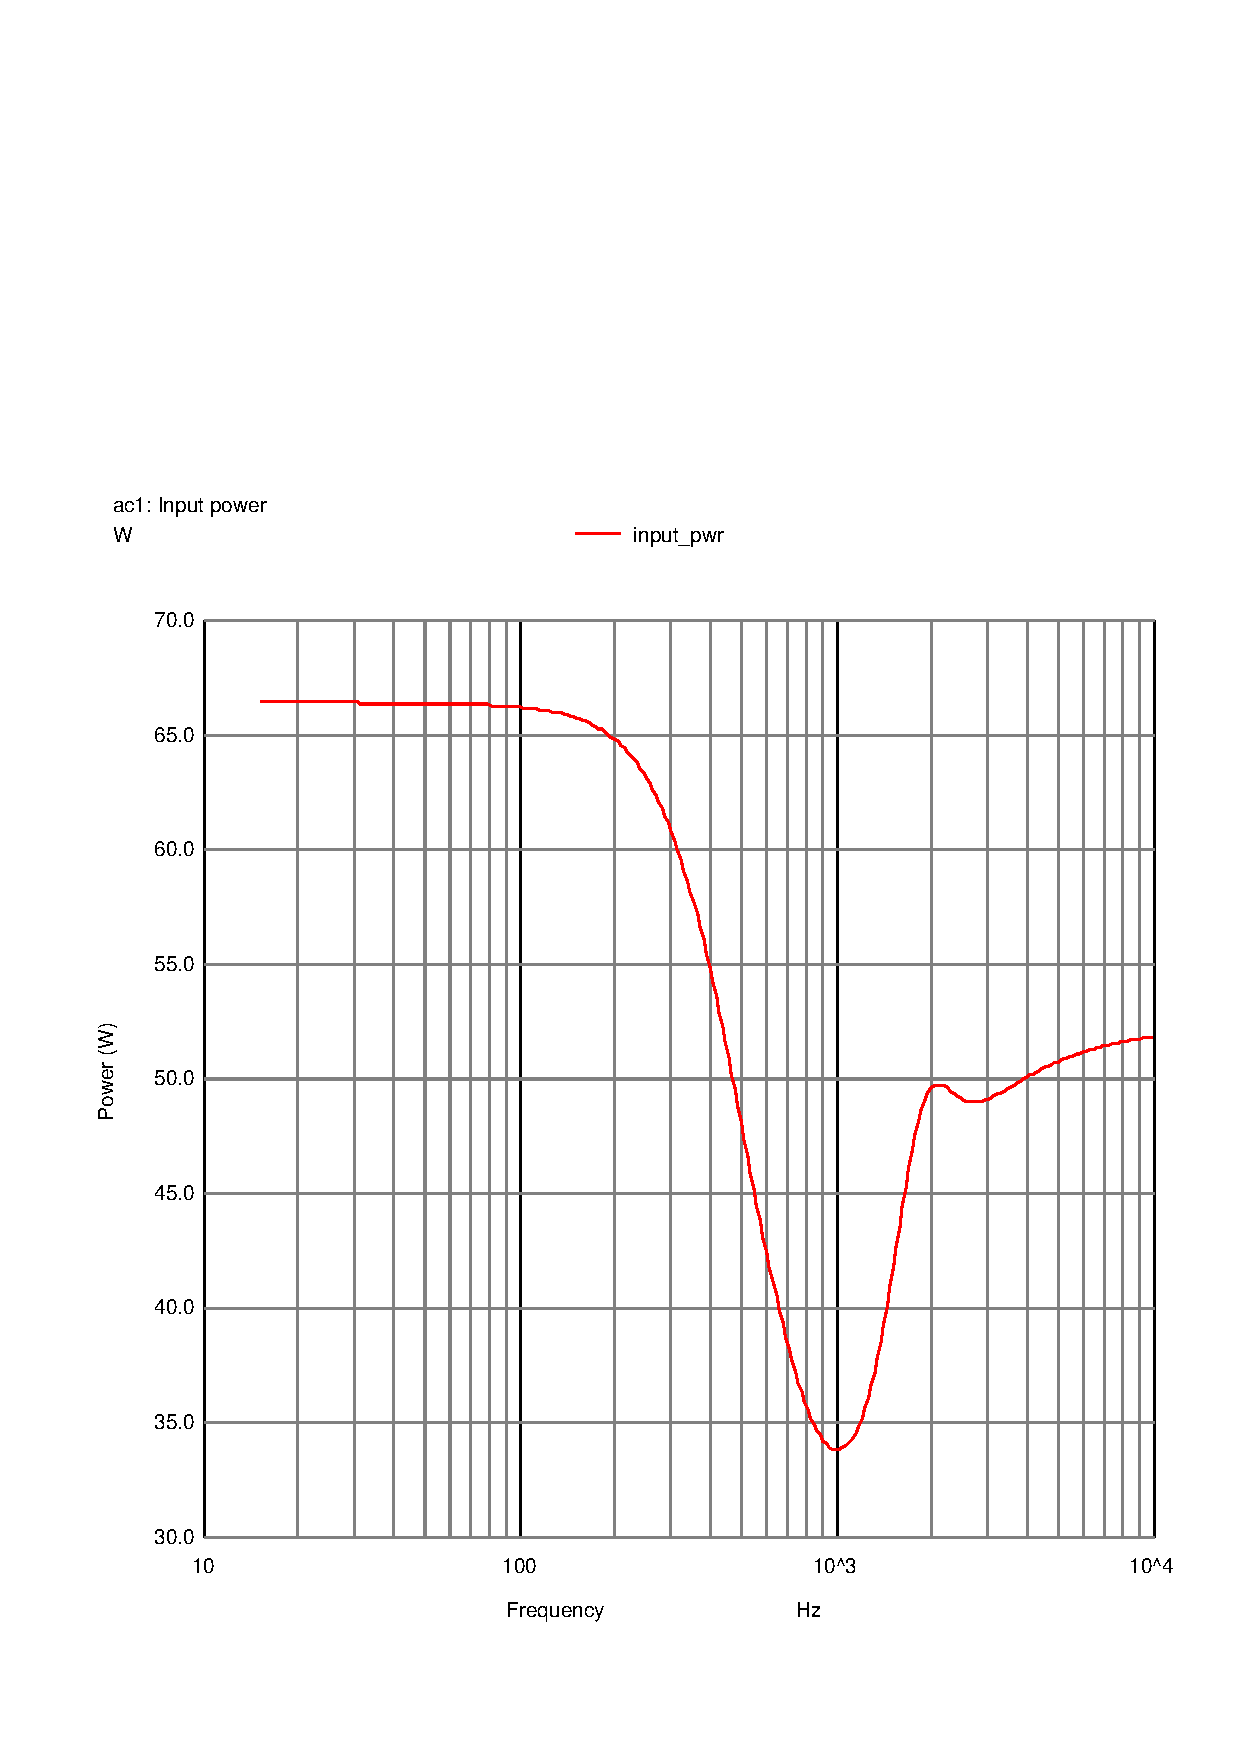
\includegraphics[scale=0.35,page=1]{../crossover/ngspice/in_pwr.pdf}
	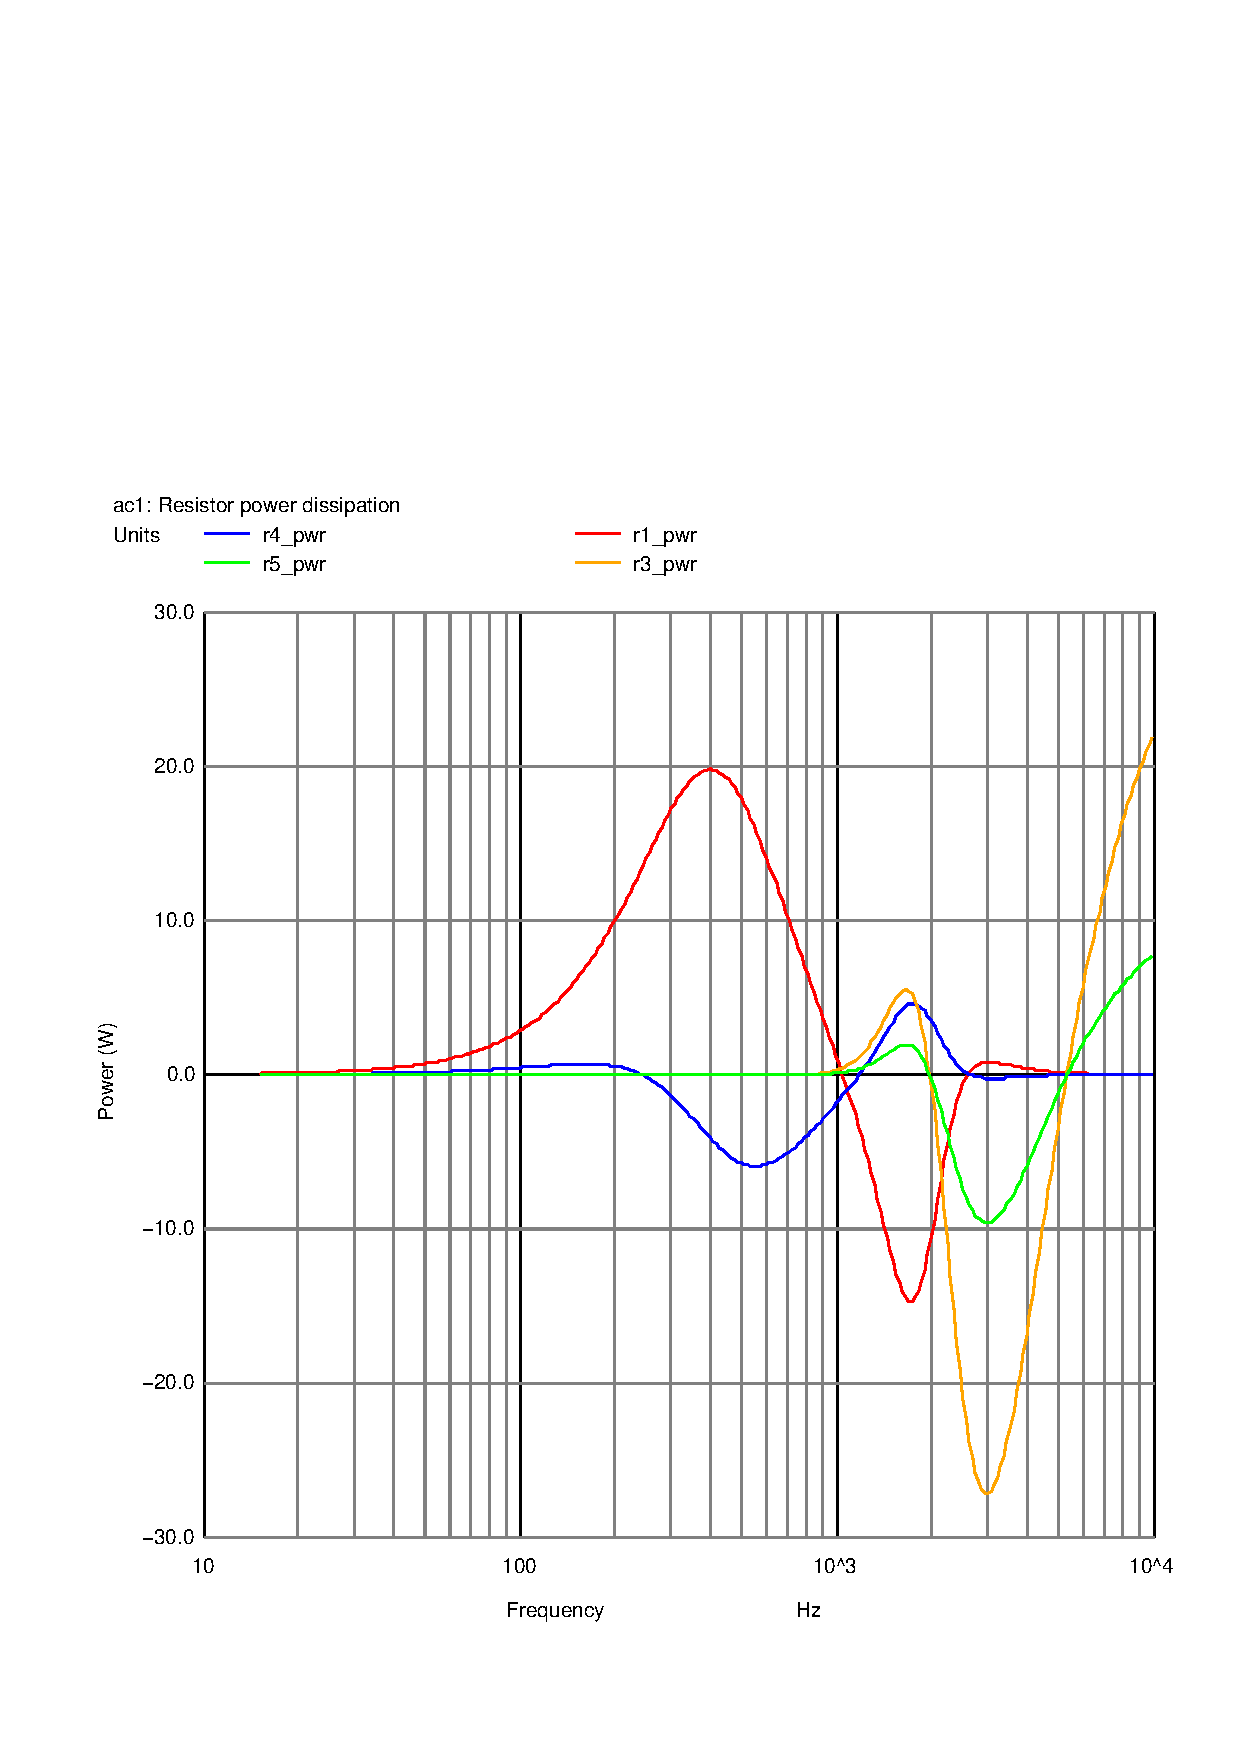
\includegraphics[scale=0.35,page=1]{../crossover/ngspice/r_pwr.pdf}
	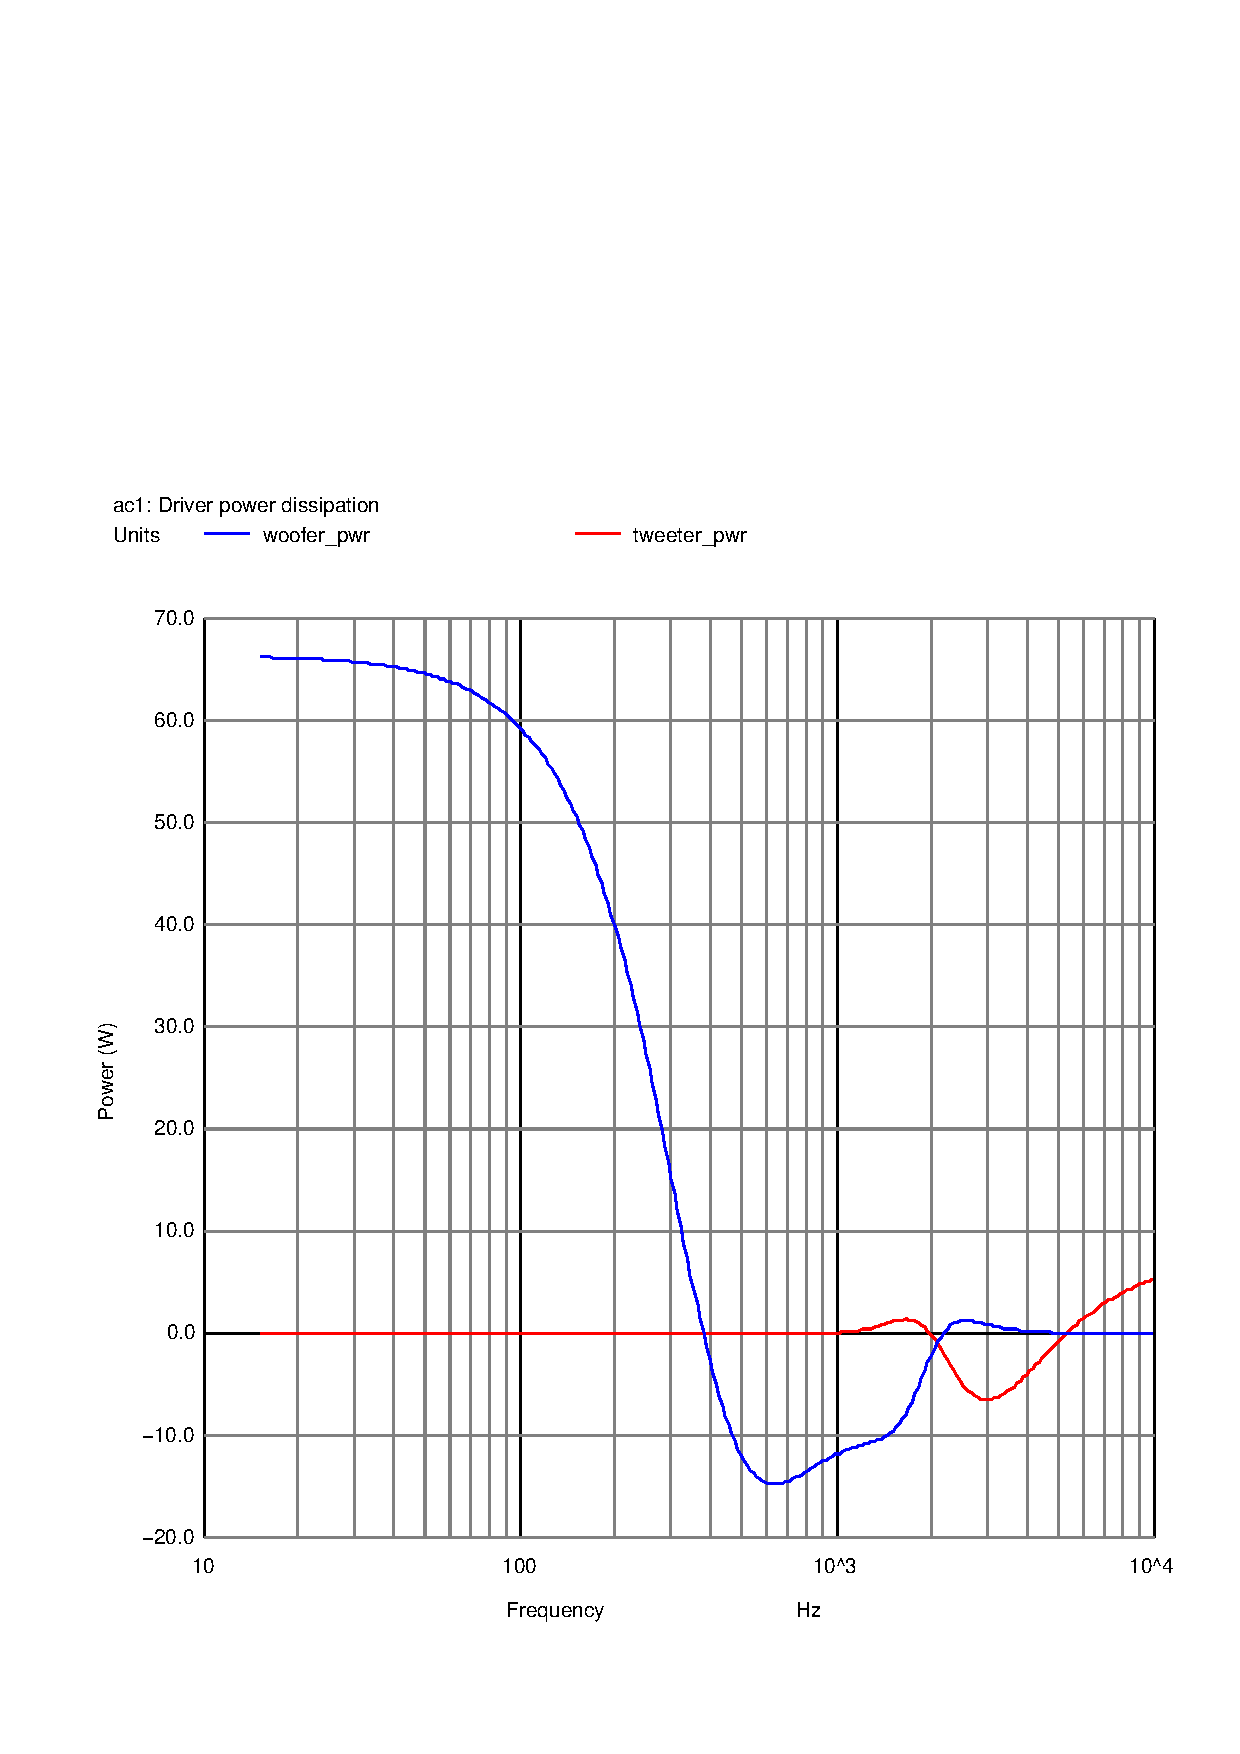
\includegraphics[scale=0.35,page=1]{../crossover/ngspice/spk_pwr.pdf}
	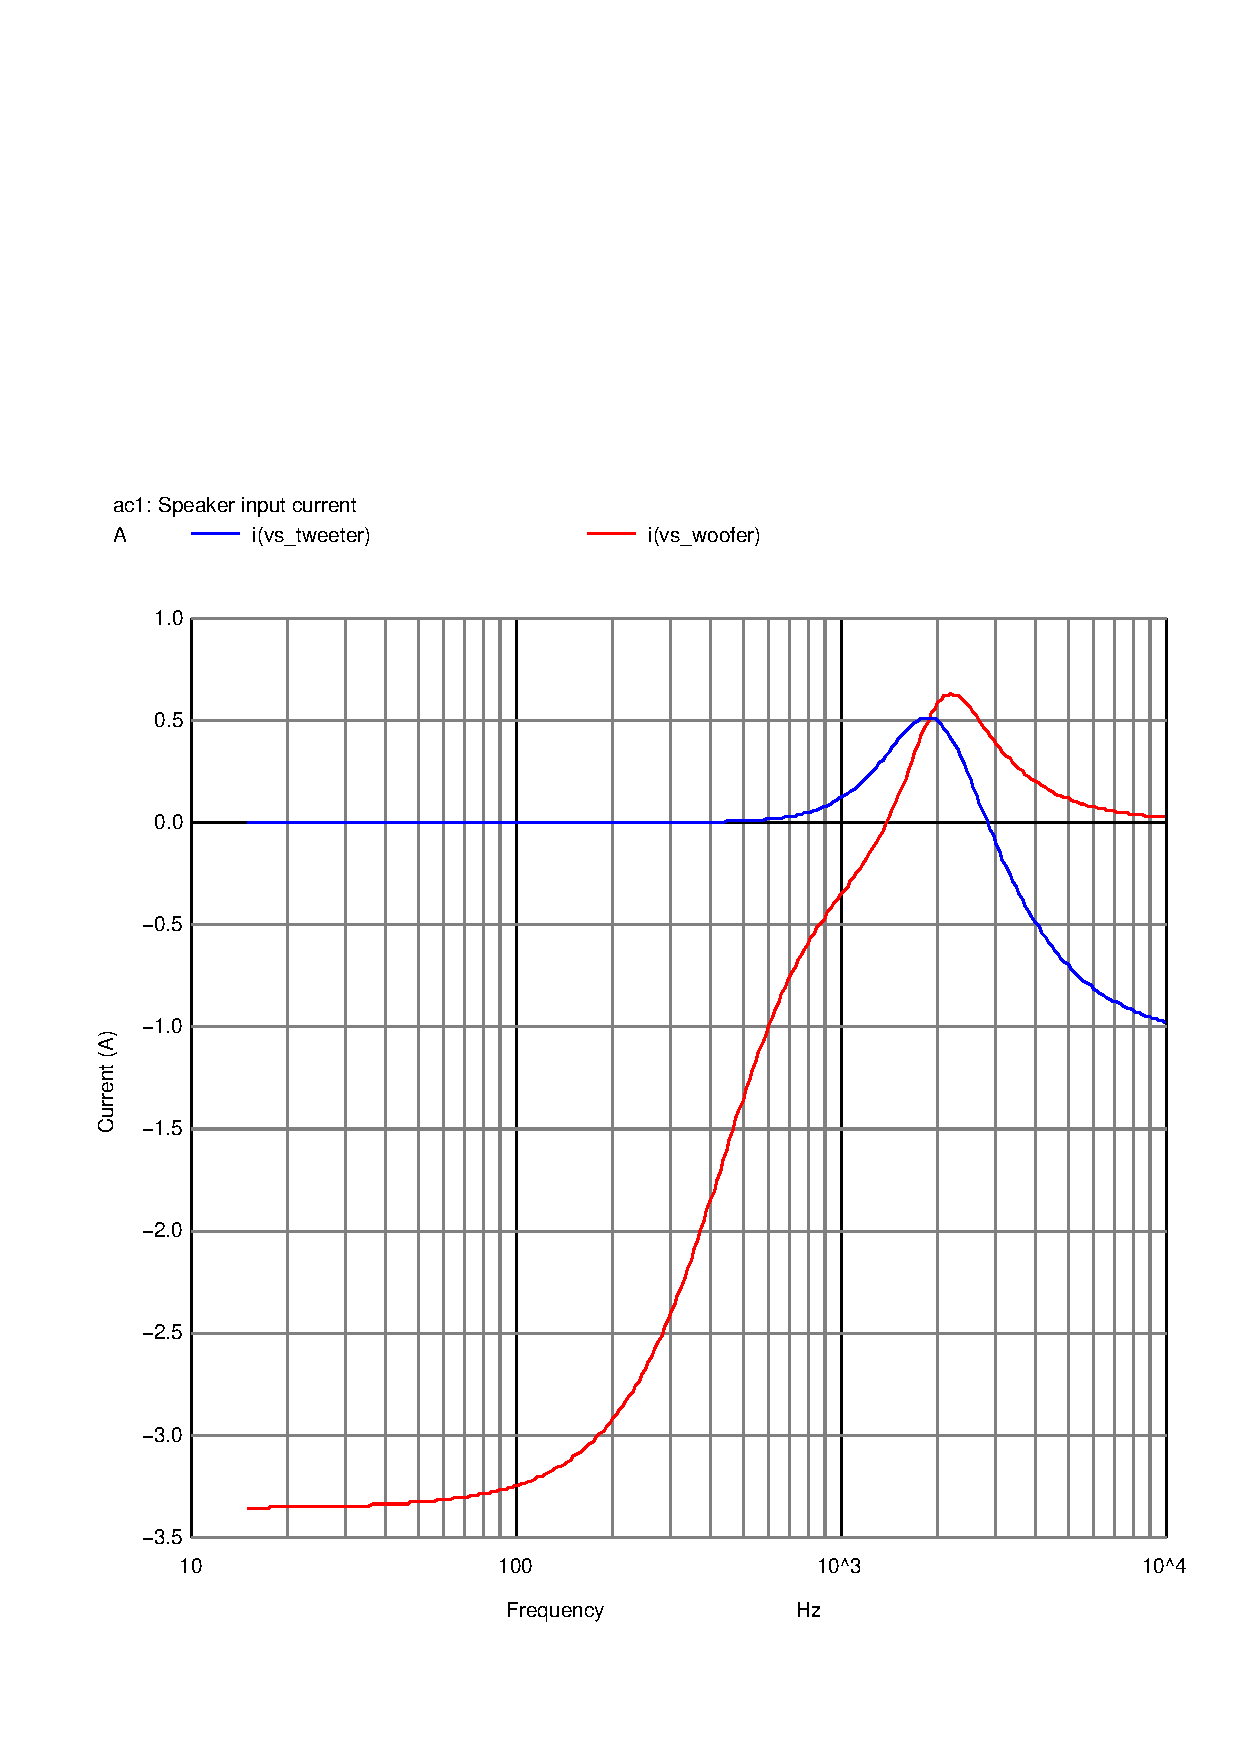
\includegraphics[scale=0.35,page=1]{../crossover/ngspice/in_current.pdf}
\end{multicols}

\end{document}
